%----------------------------------------------------%
%                    INTRODUCCION                    %
%----------------------------------------------------%

\pagestyle{fancy}

\chapter{Introducción}
\label{introduccion}

Desde Aristóteles y su libro Segundos Analíticos \footnote{\href{https://docs.google.com/a/datik.es/file/d/0By4kcbi6MzzdUHhVQnUtcTNUdk0/view}{Órganon II de Aristóteles: Recopilación de obras Aristotélicas que incluye el libro Segundo Analíticos}} hasta Galileo, padre de la ciencia moderna, adalides del conocimiento han proclamado que un método de investigación basado en lo empírico y en la medición, sujeto a los principios específicos de las pruebas de razonamiento es el camino para conocer la verdad.\\

Hoy en día, época en la que los avances tecnológicos han posibilitado observar y medir de forma exhaustiva un gran abanico de fenómenos, la ingente cantidad de datos que se genera en el proceso es, a veces, intratable mediante las tecnologías convencionales, y por ende, es imposible extraer todo el conocimiento que atesoran. El problema, lejos de atenuarse, se acrecienta con el paso del tiempo. Estudios como el realizado por McKinsey Global Institute \footnote{\href{http://www.mckinsey.com/mgi/overview}{McKinsey Global Institute}} estiman que el volumen de datos que se genera crece un 40\% cada año y auguran que entre 2009 y 2020 se verá multiplicado por 44 \cite{nambiartowards}.\\

Para lidiar con dicha problemática, en los últimos años ha irrumpido la necesidad de desarrollar nuevas metodologías y tecnologías que permitan operar eficientemente sobre masas colosales de datos, dando como resultado el nacimiento del Big Data \cite{manyika2011big}.\\

Empresas de renombre mundial, conscientes de los beneficios que el Big Data les puede reportar en diferentes facetas de su negocio, ya se han interesado en este fenómeno. De un estudio realizado entre los altos ejecutivos de las firmas que lideran el Wall Street se desprende que el 96\% tiene planeadas ciertas iniciativas relacionadas con el Big Data, y el 80\% ya tiene finalizada alguna \cite{bdes:2013}. 

\section{Contexto}
 
Datik Información Inteligente \footnote{\url{http://www.datik.es/}} es una empresa tecnológica perteneciente al Grupo Irizar \footnote{\url{http://www.irizar.com/irizar/}} que desarrolla soluciones ITS destinadas a la gestión del trasporte, tanto ferroviario como por carretera y movilidad ciudadana.\\

Uno de los productos estrella de la entidad es el denominado iPanel, concentrador de  información que ofrece al operador de transporte servicios de valor añadido en la gestión de la información generada por su flota. El funcionamiento del servicio se puede resumir mediante la Figura \ref{fig:ipanel} de la página \pageref{fig:ipanel}.

\begin{figure}[h]
	\centering
	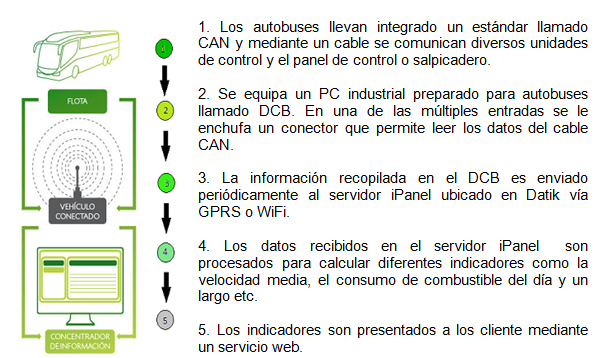
\includegraphics[width=1\textwidth]{Ilustraciones/ipanel_infraesctructure.png}
	\caption{Funcionamiento resumido de iPanel}
	\label{fig:ipanel}
\end{figure}

La incesante integración de nuevos vehículos a iPanel ha generado un crecimiento exponencial en el número de registros almacenados en ciertas tablas MySQL. Aunque el volumen actual no llega a suponer riesgo alguno para el funcionamiento del servicio, Datik tiene identificados varios escenarios en los que la situación se podría revertir, causando graves inconvenientes.\\

Fiel reflejo de ello es el Cálculo de Indicadores: proceso de ejecución diaria que realiza operaciones aritméticas intensivas sobre datos almacenados en diversas tablas, para después, agrupar los resultados en base a diferentes criterios. Siendo dichas tablas las que mayor crecimiento experimentan, el aumento del volumen de las mismas incrementa de forma desorbitada el tiempo necesario para finalizar el cálculo.\\

El objetivo del presente proyecto es proponer soluciones tecnológicas que solvente permanentemente el problema del proceso Cálculo de Indicadores y que a su vez, puedan valer para lidiar con otros obstáculos de la misma índole que pudiesen emerger en un futuro.

\section{Propuesta}

Debido a que la problemática referente al Cálculo de Indicadores es originado por el incremento exponencial de datos que dicho proceso ha de tratar, no sería descabellado pensar que la solución pudiese pasar por escalar verticalmente la máquina y/o afinar la configuración del servicio MySQL ya existente. No obstante, ambas mejoras son limitadas, mientras que el volumen de los datos seguiría en aumento de forma inexorable.\\

Siendo imposible reconducir la situación mediante el uso de las tecnologías tradicionales, en el presente proyecto se propone realizar un cambio de paradigma y migrar a un modelo distribuido que posibilite escalar la infraestructura horizontalmente. A su vez, se sugiere dividir el problema en dos apartados, almacenamiento y procesamiento, dotando la infraestructura de tecnología adecuada para ofrecer una respuesta eficaz a cada una de las facciones.\\

En cuanto a almacenamiento se refiere, debido a la imperante necesidad de escarbar en hercúleos volúmenes de datos, se propone utilizar una base de datos no relacional. Dentro de la extensa y heterogénea gama de sistemas de almacenamiento NoSQL \footnote{\url{http://nosql-database.org/}} existentes a día de hoy, se ha considerado idóneo el uso de Apache Cassandra \cite{lakshman2010cassandra}, una base de datos distribuida del tipo clave-valor que ofrece alta disponibilidad sin un solo punto de fallo, un ratio de escrituras por segundo sustancialmente superior en comparación a sus homólogos \cite{rabl2012solving} y velocidades de lectura nada desdeñables.\\

Por su parte, la tecnología seleccionada para el procesamiento ha sido Apache Spark \cite{zaharia2010spark}, una plataforma de computación en clúster que ofrece una interfaz para programar operaciones paralelizadas y tolerantes a fallo que ha irrumpido con fuerza en el último lustro. A logrado desbancar tecnologías semejantes como MapReduce \cite{dean2008mapreduce} gracias a la capacidad de almacenar en memoria los resultados intermedios del cómputo posibilitando así acelerar el procesamiento hasta 100 veces \cite{xin2013shark} en determinados escenarios.\\

Para cuantificar los beneficios aportados por las tecnologías propuestas se ha decidido utilizar un Dataset público de aproximadamente 25 GB que recoge la información de los trayectos realizados por los taxis amarillos de Nueva York durante el año 2015\footnote{\url{http://www.nyc.gov/html/tlc/html/about/trip_record_data.shtml}}, ya que los datos actualmente almacenados por Datik se encuentran sujetos a una cláusula de confidencialidad.

\section{Organización del documento}

El presente documento abarca el estudio empírico realizado sobre el rendimiento obtenido mediante el uso conjunto de Apache Cassandra y Apache Spark en comparación al ofrecido por MySQL Server en escenarios que requieren un almacenamiento y procesamiento eficaz de volúmenes masivos de datos.\\

En este primer capítulo, se ha introducido la problemática que ha impulsado la creación del proyecto y expuesto la propuesta tecnológica para dar solución a la misma.\\

En el capítulo 2, se desgrana el funcionamiento de las tecnologías electas para resolver el problema, haciendo especial hincapié en las peculiaridades que les permiten ofrecer una mejora sustancial en comparación a otras herramientas.\\

Una vez en el capítulo 3, se detalla la praxis llevada a cabo para confeccionar los dos entornos de prueba. Por un lado, se describe la construcción de un entorno centralizado compuesto por un único nodo que alberga una instancia de MySQL y por el otro, la de uno distribuido, formado por tres nodos homogéneos sobre el cual operan Apache Cassandra y Apache Spark en consonancia.\\ 

El almacenamiento y la retribución de los datos constituyen el grueso del 4to capítulo. Primero, se expone la naturaleza de los datos que conforman el data-set y se enuncian las consultas que se desean realizar sobre este. Después, se presenta el diseño de las tablas utilizadas para almacenar dichos datos, incidiendo especialmente en la correspondiente a Apache Cassandra debido a las peculiaridades que presenta.\\ 

En el capítulo 5, se publican los resultados obtenidos una vez habiendo ejecutado las consultas anteriormente definidas. Dichos resultados son representados mediante gráficas y analizados posteriormente para observar de forma nítida las diferencias existentes entre ambos entornos.\\

Para finalizar, en el capítulo 6 se presentan las conclusiones y líneas futuras para el proyecto.\\

Fuera de la estructura general de la memoria, se puede encontrar la bibliografía citando todas las fuentes relevantes accedidas en el devenir del presente trabajo.